% METODOLOGIA------------------------------------------------------------------

\chapter{Implementação do Protótipo}
\label{chap:prototipo}

Este capitulo descreve a montagem do protótipo para testes. Será feita uma introdução do funcionamento geral, e suas principais características. Posteriormente, será mostrado o funcionamento da base de testes da câmera, conexões entre os servo motores e os pinos GPIOs (\textit{General-Purpose Input/Output}) do \textit{Raspberry Pi}, desenvolvimento do programa de controle dos servo motores, desenvolvimento do aplicativo \textit{Android}, responsável por capturar dados dos sensores de posição e envia-los pela rede sem fio.

\section{Conceito}
\label{sec:conceito}

A ideia central do projeto é trazer ao operador de um robô de inspeção, um controle intuitivo para câmera embarcada. Pretende-se criar a sensação de imersividade, isto é, projetar o operador no ambiente inspecionado, através da visão \textit{stereo}, simulada no protótipo por apenas uma câmera, e a tradução dos movimentos da cabeça do operador em movimentos da câmera embarcada.\par
Para atingir este objetivo, um celular será acoplado a cabeça do operador, através de um óculos VR (Google \textit{cardboard}), ilustrado na \autoref{fig:googlecardboard}. Prende-se o óculos a cabeça por uma alça, fixada com \textit{Velcro}, indicado com as marcações verdes da \autoref{fig:googlecardboard_welcro}. \par 

\begin{figure}[H]
	\centering
	\begin{subfigure}{.5\textwidth}
		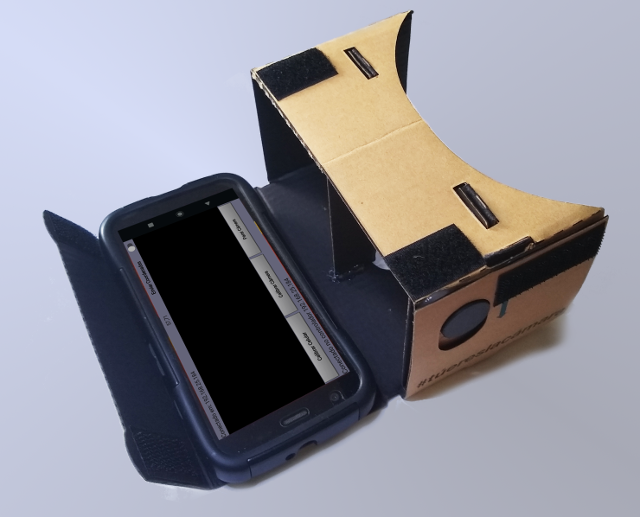
\includegraphics[width=0.95\textwidth]{figuras/cardboard1.png}
		\caption{visão fontal (compartimento do celular).}
	\end{subfigure}%
	\begin{subfigure}{.5\textwidth}
		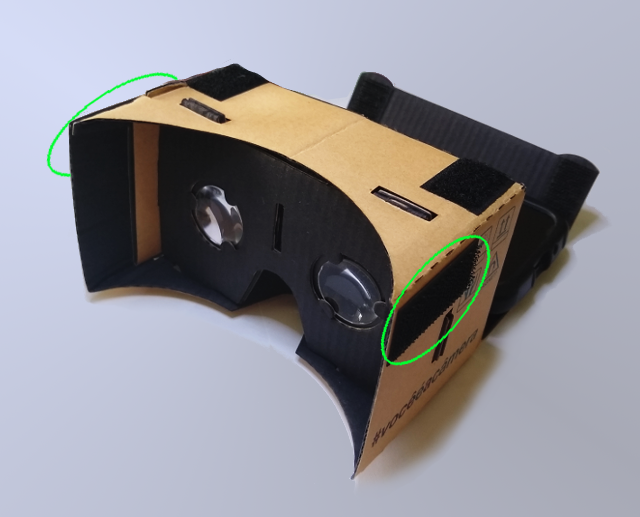
\includegraphics[width=0.95\textwidth]{figuras/cardboard2.png}
		\caption{visão traseira (lentes).}
		\label{fig:googlecardboard_welcro}
	\end{subfigure}
	\caption{Google Cardboard.}
	\label{fig:googlecardboard}
\end{figure}

Os sensores do celular capturam os movimentos rotacionais da cabeça do operador, como mostra a sequencia da \autoref{fig:headmotion}, e os enviam para o centro de controle, um \textit{Raspberry Pi} embarcado junto com uma câmera e seus atuadores.\par

\begin{figure}[H]
	\centering
	\begin{subfigure}{.5\textwidth}
		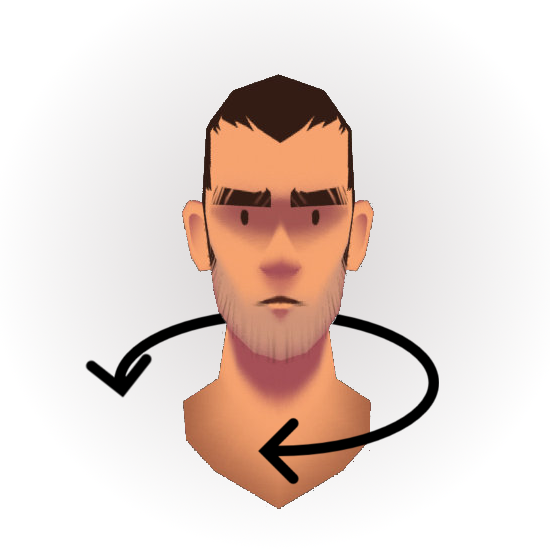
\includegraphics[width=0.95\textwidth]{figuras/yaw.png}
		\caption{rotação horizontal (\textit{yaw}).}
		\label{fig:headmotion_yaw}
	\end{subfigure}%
	\begin{subfigure}{.5\textwidth}
		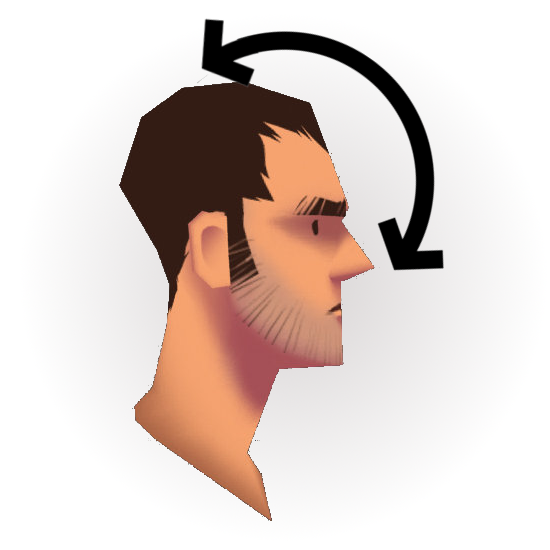
\includegraphics[width=0.95\textwidth]{figuras/pitch.png}
		\caption{rotação vertical (\textit{pitch}).}
		\label{fig:headmotion_pitch}
	\end{subfigure}
	\caption{Movimentos de rotação da cabeça do operador.}
	\fonte{\citeonline{kieranlampert2019} Modificado}
	\label{fig:headmotion}
\end{figure}

Os movimentos, indicados na \autoref{fig:headmotion}, são traduzidos em movimentos \textit{pan} e \textit{tilt} da câmera, como ilustrado na \autoref{fig:cameramotion}.

\begin{figure}[H]
	\centering
	\begin{subfigure}{.5\textwidth}
		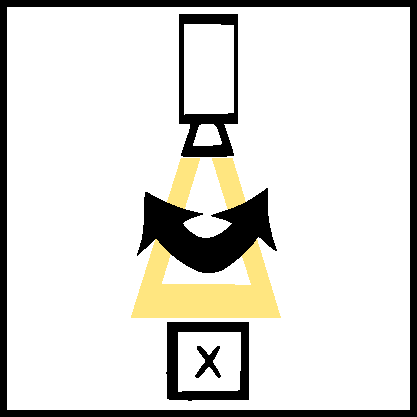
\includegraphics[width=0.90\textwidth]{figuras/Pan1.pdf}
		\caption{visão superior de uma câmera,\newline indicando o movimento horizontal (\textit{pan}).}
		\label{fig:cameramotion_pan}
	\end{subfigure}%
	\begin{subfigure}{.5\textwidth}
		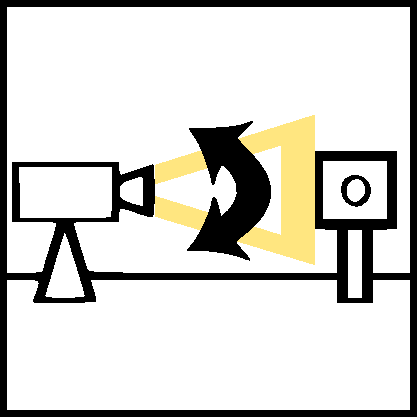
\includegraphics[width=0.90\textwidth]{figuras/Tilt1.pdf}
		\caption{visão lateral de uma câmera,\newline indicando movimento vertical (\textit{tilt}).}
		\label{fig:cameramotion_tilt}
	\end{subfigure}
	\caption{Movimentos da Câmera.}
	\fonte{\citeonline{publicdomain2019} Modificado}
	\label{fig:cameramotion}
\end{figure}

\section{Especificação do Projeto}
\label{sec:especificacao}

O projeto pode ser dividido conceitualmente em duas partes, denominadas por: \textbf{Módulo de Controle de Câmera (MCC)}, o \textit{Raspberry Pi} e \textbf{Módulo de Captura de Movimento (MCM)}, o \textit{smartphone} \textit{Android}. O MCC é responsável por receber os dados de posição através de uma conexão \textit{socket}, converter o sistema de coordenadas, aplicar um filtro para evitar o acionamento desnecessário dos motores, impedindo o aquecimento, e acionar os servos. O MCM é responsável por configurar os sensores de localização disponíveis no \textit{smartphone}, aplicar os filtros necessários para minimizar ruídos na coleta de dados, configurar automaticamente uma conexão \textit{socket} com MCC, através de uma busca na rede, e enviar dados das coordenadas. \par

\begin{figure}[H]
	\centering
	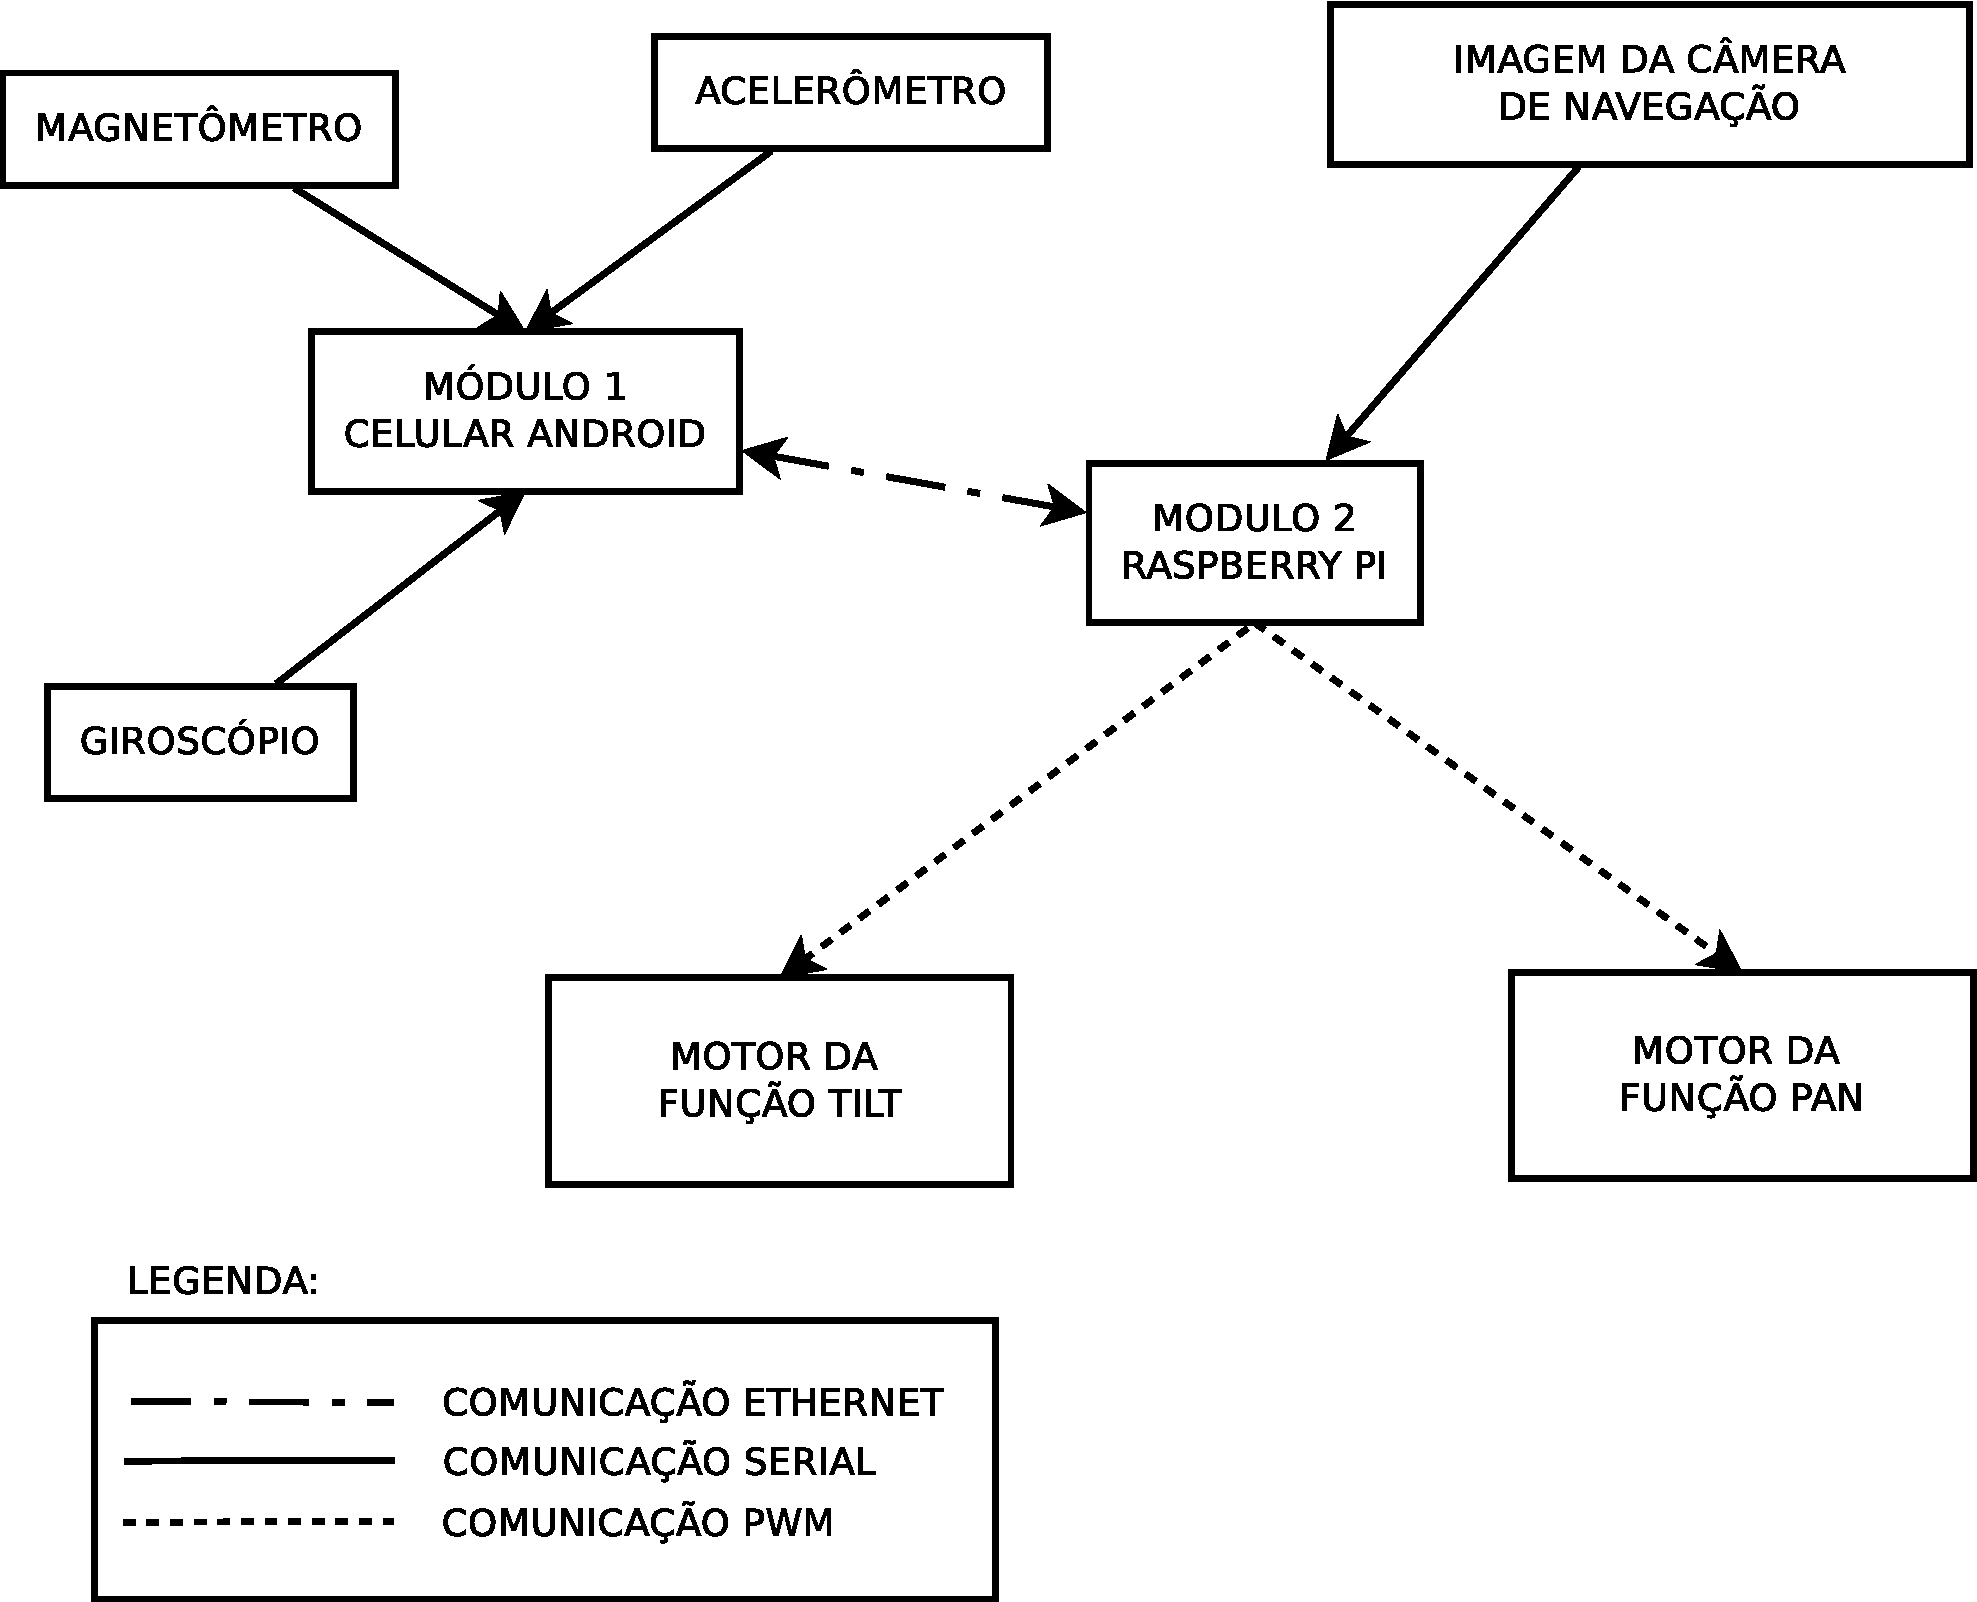
\includegraphics[trim={6cm 3cm 5cm 3cm},clip,width=0.8\textwidth]{figuras/diagrama-modulos-eps-converted-to.pdf}
	\caption{Diagrama de blocos da comunicação entre os principais componentes da solução}
	\label{fig:diagrama_blocos}
\end{figure}

A \autoref{fig:diagrama_blocos} ilustra a comunicação entre os módulos, sensores e atuadores. Os sensores estão embarcados no smartfone e não serão controlados separadamente, sendo automático o seu acionamento. O sistema operacional \textit{Android} fornece uma abstração para o hardware, e portanto não será necessário configurar os sensores manualmente.

\subsection{Módulo de Controle de Câmera (MCC)}
\label{subsec:modconcam}

O Módulo de Controle de Câmera consiste em um SoC \textit{Raspberry Pi} 1 modelo B, que possui um processador ARM de 700MHz, 512Mb de memória RAM, 26 pinos de proposito geral (GPIO), dua portas USB e uma porta Ethernet. O MCC tem as seguintes responsabilidades:

\begin{itemize}
	\item Responder requisições \textit{broadcast} particulares, que identificam o MCM
	\item Receber dados de posição de sensores
	\item Filtrar os dados recebidos para evitar acionamento desnecessário dos motores
	\item Traduzir coordenadas dos sensores para coordenadas das câmeras
	\item Acionar dois motores servos de acordo coordenadas recebidas
	\item Iniciar o serviço de \textit{stream} de video
	\item Finalizar o serviço de \textit{stream} de video
	\item Calibrar a posição da câmera (salvar posição corrente e usar esse dado para os próximos movimentos)
\end{itemize}

\subsection{Módulo de Captura de Movimento (MCM)}
\label{subsec:modcapmov}

O Módulo de Captura de Movimento é um smartfone \textit{Android} Motorola G6 com processador, de arquitetura ARM, modelo \textit{Qualcomm} \textit{Snapdragon 450}, com 8 núcleos (Octa-Core), com \textit{clock} de 1,8 GHz, 3GB de memória RAM, conectividade \textit{Wi-Fi}, que possui os seguinte sensores: Acelerômetro, Magnetômetro, Giroscópio, Proximidade, Luz Ambiente e leitor de Impressão Digital. O MCM é responsável por:

\begin{itemize}
	\item Enviar requisição \textit{broadcast} especial para detectar o MCC
	\item Conectar no MCC
	\item Configurar a orientação do dispositivo em relação aos eixos de referencia (\autoref{fig:axisdevice} e \autoref{fig:axisglobe})
	\item Coletar dados dos sensores de movimento
	\item Aplicar filtros nos dados obtidos dos sensores
	\item Enviar coordenadas para o módulo de controle de câmera
	\item Mostrar vídeo capturado pela câmera do MCC em formato \textit{stereo}
	\item Mostrar informações pertinentes ao estado do MCC, como o endereço IP (\textit{Internet Protocol}) configurado
\end{itemize}

\section{Montagem do Protótipo}
\label{sec:assemprototipo}

O protótipo foi construído usando uma PSU (\textit{Power Supply Unit}) de computador de mesa, padrão ATX (\textit{Advanced Technology eXtended}), como fonte de alimentação e suporte de montagem para todos os componentes, com exceção do \textit{smartphone}.\par

Cola quente foi usada para fixar à base (e fonte de energia), o \textit{Raspberry Pi}, corpo de montagem da câmera com motores servos (suporte articulado) e um ponto de acesso sem fio, que fornece a infra-estrutura de rede para o projeto. \par

O suporte dos motores servo e da câmera é uma estrutura moldada em plástico, ilustrado na \autoref{fig:basedesmontada}, que precisa ser montada com parafusos. A posição de descanso dos motores (centro de curso) precisa ser regulada neste momento, não sendo possível modificar está posição facilmente depois que o suporte estiver montado, ilustrado na \autoref{fig:basemontada}.\par

\begin{figure}[H]
	\centering
	\begin{subfigure}{.5\textwidth}
		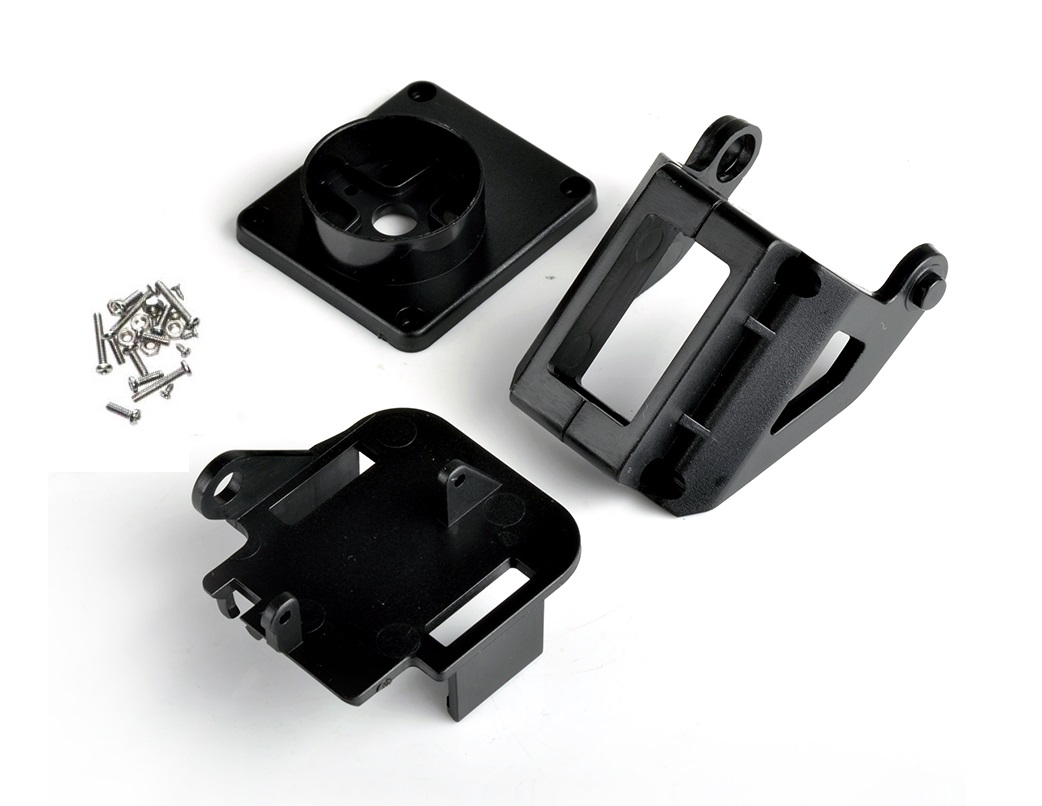
\includegraphics[width=0.95\textwidth]{figuras/base2.jpg}
		\caption{Componentes do suporte.}
		\label{fig:basedesmontada}
	\end{subfigure}%
	\begin{subfigure}{.5\textwidth}
		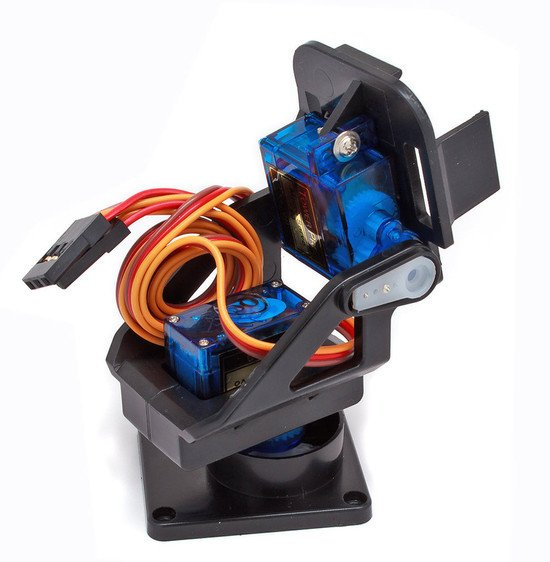
\includegraphics[width=0.75\textwidth]{figuras/base3.jpg}
		\caption{Montagem com motores.}
		\label{fig:basemontada}
	\end{subfigure}
	\caption{Base de suporta para motores e câmera.}
\end{figure}

Com a intensão de testar os motores, e preservar o \textit{Raspberry Pi} (um dispositivo menos tolerante a falhas, quando se trata de níveis de tensão nos pinos GPIO), foi desenvolvido um circuito gerador de sinal PWM (\textit{Pulse width modulation}), também conhecido como \textbf{\textit{driver} PWM}, ilustrado na \autoref{fig:pwmtestcircuit}. O circuito permitia ajustar tanto a frequência do sinal quanto a largura dos pulsos, através de ajustes no potenciômetro POT3 e de um resistor que substituiu os potenciômetros POT1 e POT2 no circuito real, implementado na \textit{breadboard}. Utilizando o circuito foi possível identificar a posição central dos motores e verificar sua estabilidade, enquanto se variava a frequência do sinal. O drive foi montado usando o circuito integrado NE555, um componente eletrônico bastante usado em aplicações que envolve temporização, geração de pulso e PWM. \par

\begin{figure}[H]
	\centering
	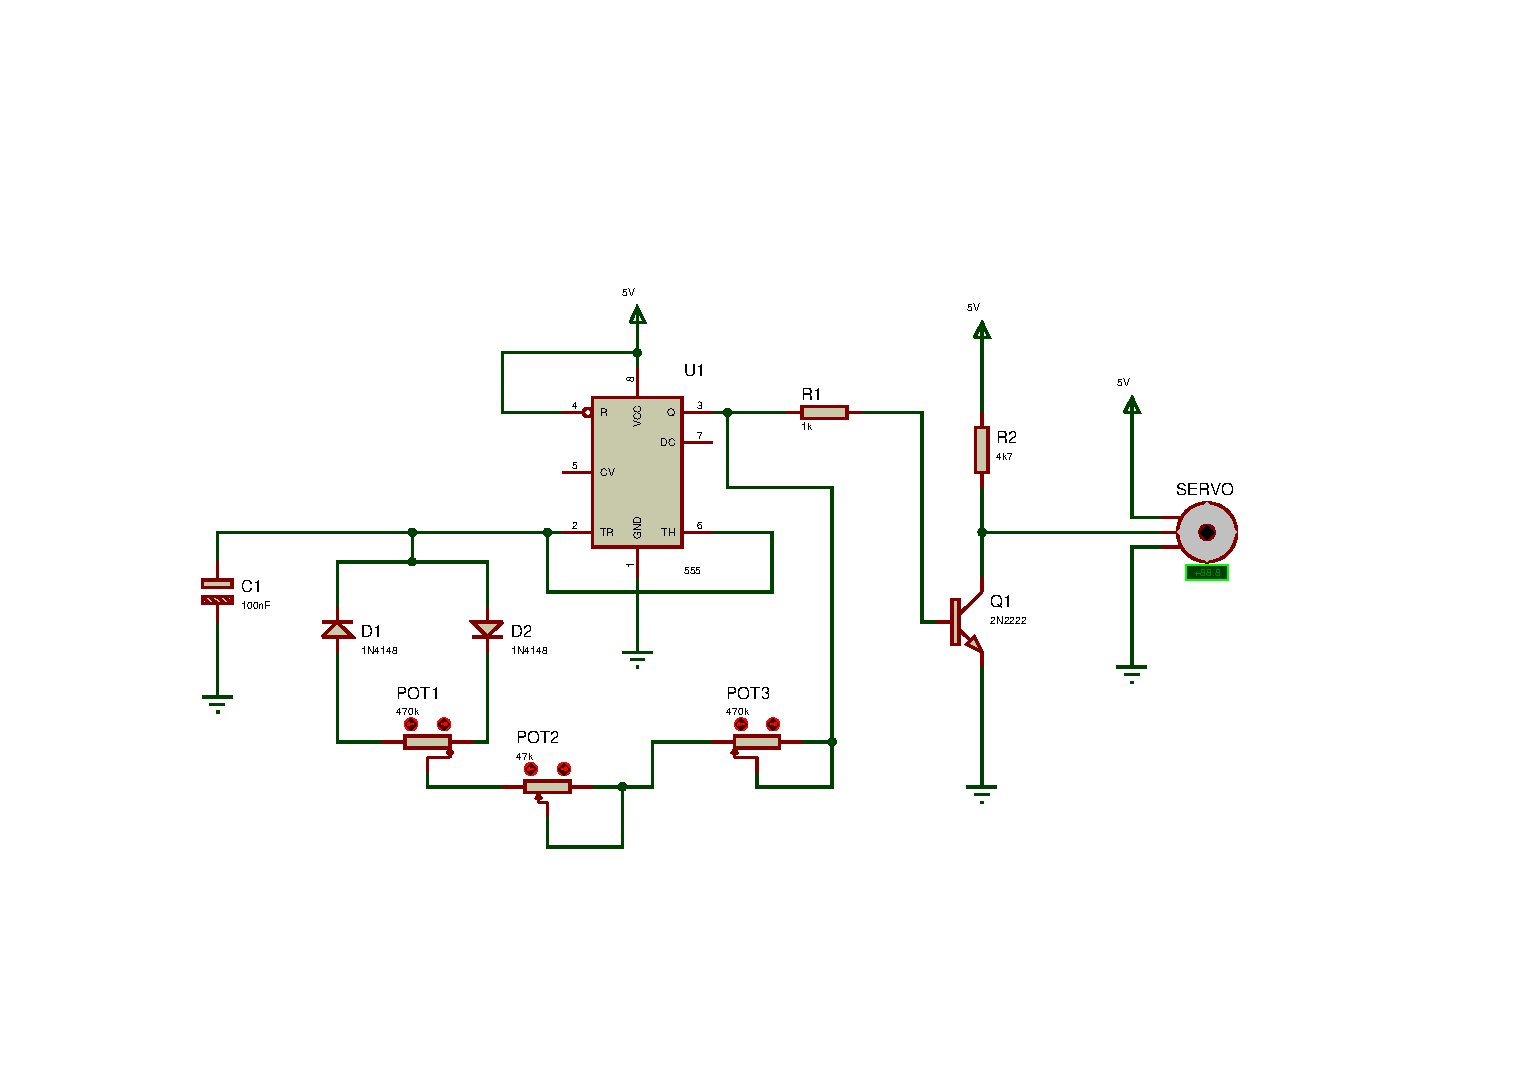
\includegraphics[trim={2.5cm 3cm 4cm 5cm},clip,width=1\textwidth]{figuras/pwm2.pdf}
	\caption{\textit{Driver} PWM de teste.}
	\label{fig:pwmtestcircuit}
\end{figure}

Ativando individualmente os motores com o \textit{driver} construído e com o auxilio de um osciloscópio, foi possível notar que os motores operam de forma estável com pulsos gerados numa frequência de 50Hz, e que é possível controlar a sua posição variando a largura do pulso entre valores próximos a 1ms, posição de angulo $180\degree$ (ângulo máximo), e valores próximos 2ms, posição de angulo $0\degree$ (ângulo mínimo), como ilustrado na \autoref{fig:pwmservo}. Foi possível observar também que existe uma correspondência linear entre a largura do pulso e a posição angular do eixo do motor, sendo assim, a posição de repouso ou centro, pode ser alcançada com uma largura de pulso próximo a 1,5 milissegundos. 

\begin{figure}[H]
	\centering
	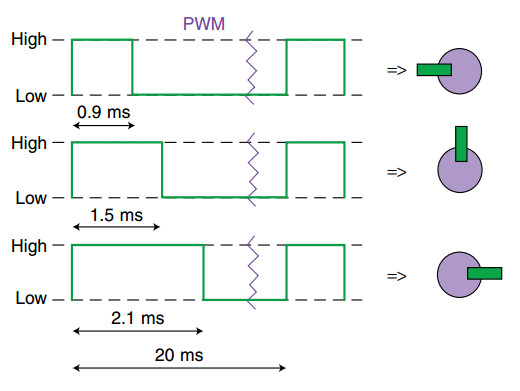
\includegraphics[width=0.7\textwidth]{figuras/pwm_servo.jpg}
	\caption{Posição do eixo do motor em função da largura de pulso PWM.}
	\fonte{\citeonline{pinckney2006pulse}}
	\label{fig:pwmservo}
\end{figure}

Para conectar os motores ao módulo de câmera \textit{Raspberry Pi}, foi necessário construir um circuito de acionamento dos motores, que consiste em dois transistores bipolares de junção (BJT 2N2222), um para cada motor, configurados no modo emissor-comum, funcionando como um interruptor acionado pelo sinal PWM gerado pelos pinos GPIO do \textit{Raspberry Pi}. A fonte do sinal PWM foi ligada ao terminal base do transistor através de um resistor de 1K$\Omega$, com a função de limitador de corrente $I_b$ e a via de sinal do motor, foi conectado ao terminal coletor do transistor juntamente a uma fonte de 5V através de um resistor de 10K$\Omega$, responsável por limitar a corrente $I_c$, máxima quando o transistor está ativado, como ilustrado no circuito da \autoref{fig:circprotecao}.\par

Esse circuito foi construído numa mini \textit{breadboard} e tem o objetivo proteger o \textit{Raspberry Pi}, evitando o consumo excessivo de corrente (mais que 15mA), ou uma possível corrente de retorno para um dos pinos GPIO, numa eventual falha do circuito interno de controle dos motores. Como o circuito de proteção inverte o sinal PWM, foi necessário gerar um sinal invertido no MCC, para que esse fosse invertido novamente pelo circuito de proteção e assim chegar como devido ao circuito de controle interno do motor.\par

A alimentação dos motores é fornecida por um outro circuito composto por um regulador linear de tensão, o LM7805, e dois capacitores, ilustrado na \autoref{fig:circfonte}, que reduz a tensão de 12V, fornecida pela PSU, pra 5V. A linha de 12V foi usada para isolar as fontes de alimentação dos motores e do \textit{Raspberry Pi}, para evitar ruídos causados pelo acionamento dos motores.

\begin{figure}[H]
	\centering
	\begin{subfigure}{.5\textwidth}
		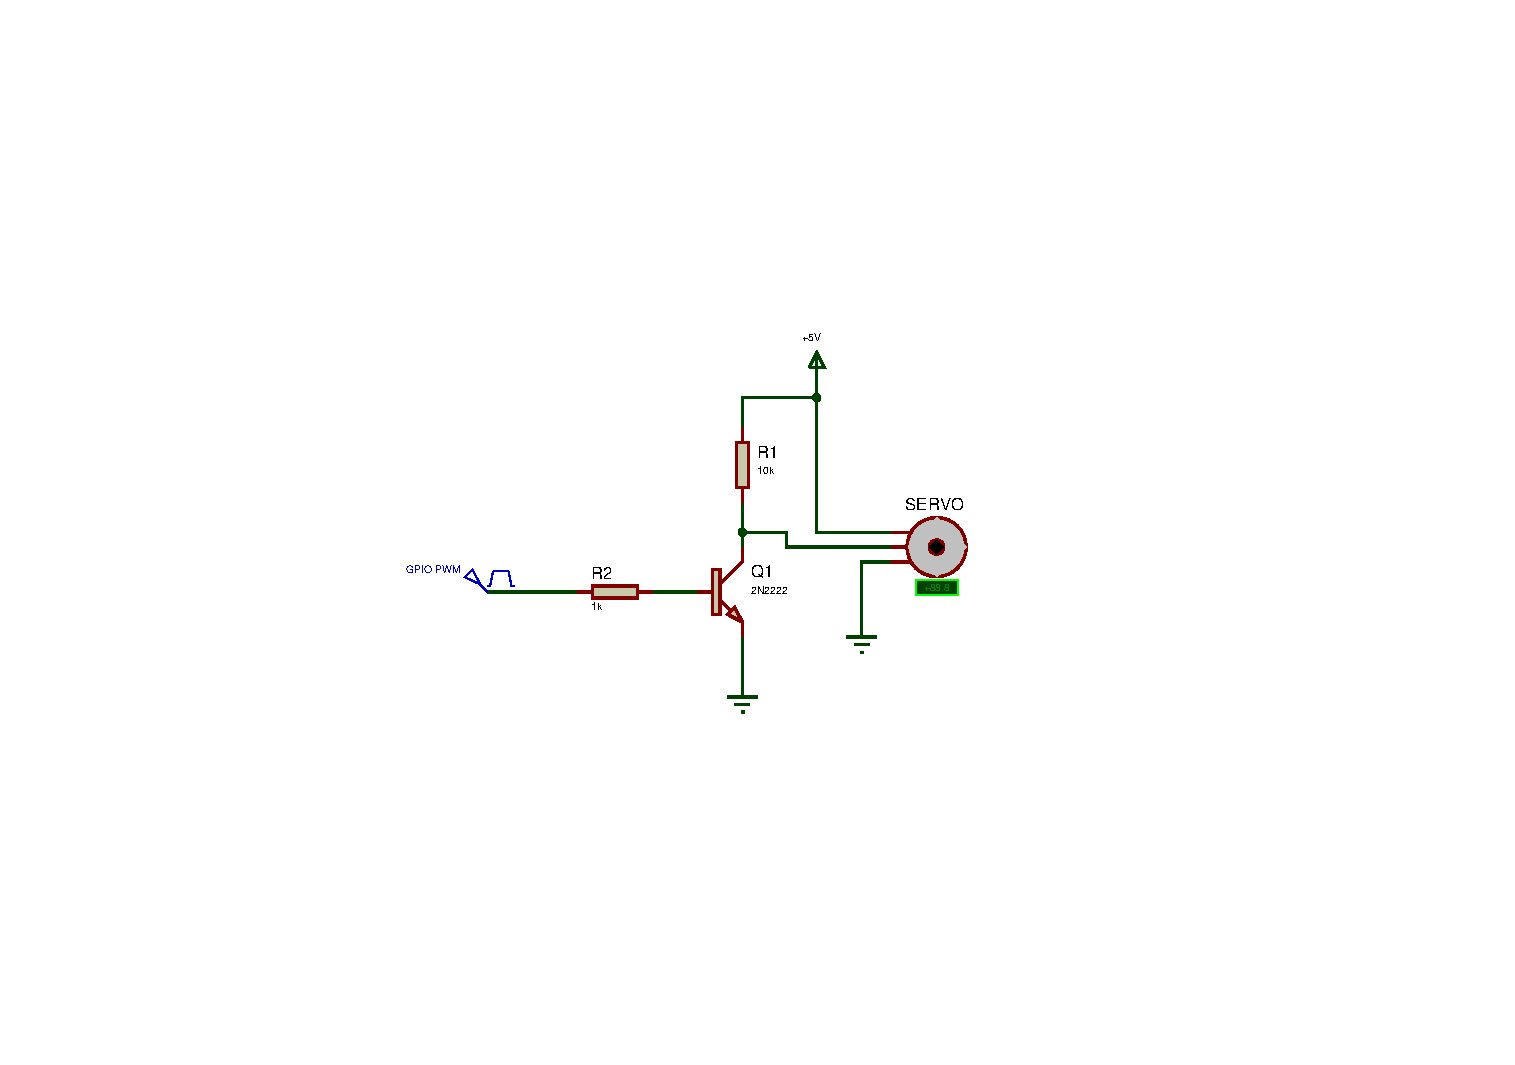
\includegraphics[trim={6.5cm 5cm 9cm 5cm},clip,width=0.9\textwidth]{figuras/circ_acionamento.pdf}
		\caption{Acionamento de motores.}
		\label{fig:circprotecao}
	\end{subfigure}%
	\begin{subfigure}{.5\textwidth}
		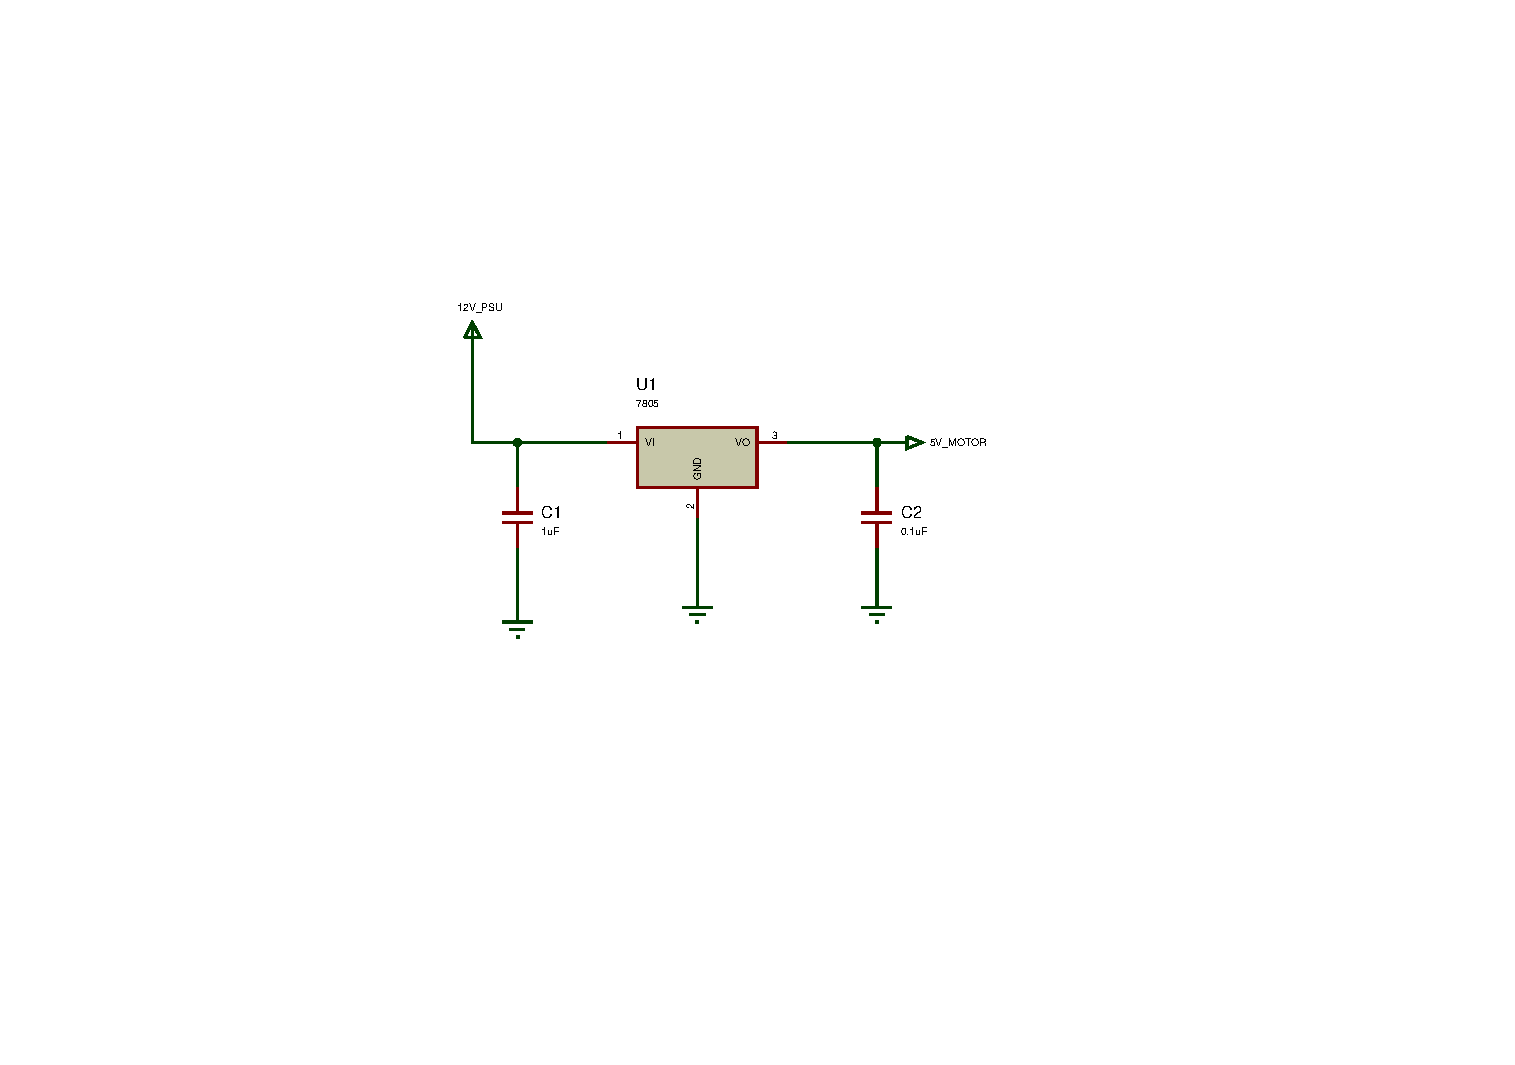
\includegraphics[trim={6.5cm 5cm 8.5cm 4cm},clip,width=0.9\textwidth]{figuras/fonte_motores.pdf}
		\caption{Regulador de tensão.}
		\label{fig:circfonte}
	\end{subfigure}
	\caption{Circuitos usados pelos motores.}
\end{figure}

\subsection{Construção do Módulo de Controle de Câmera - MCC}
\label{subsec:assemmodconcam}

O MCC é responsável por acionar os motores, usados para movimentar a câmera, e iniciar um serviço de \textit{stream} de mídia, que disponibiliza na rede usando um protocolo de tempo real, as imagens capturadas pela câmera.\par

O software de controle foi construído, usando a linguagem C, para receber valores de coordenadas enviados por uma conexão \textit{socket} e acionar os motores.\par

O MCC possui dois modos de operação, um modo de produção, que opera consumindo recursos mínimos de memória e processador, e um modo de depuração/teste, habilitado através da diretiva \textbf{\textit{\#define TEST\_DISPLAY}} ou diretamente pelo \textit{script} \textit{Makefile} passando o parâmetro \textbf{\textit{CFLAGS=-DTEST\_DISPLAY}}.
\begin{figure}[H]
	\centering
	\begin{subfigure}{.5\textwidth}
		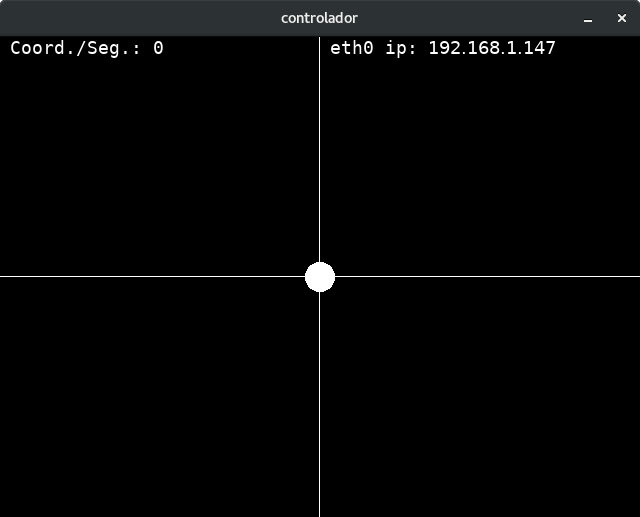
\includegraphics[width=0.95\textwidth]{figuras/controlador.jpg}
		\caption{iniciado.}
		\label{fig:controlador_teste}
	\end{subfigure}%
	\begin{subfigure}{.5\textwidth}
		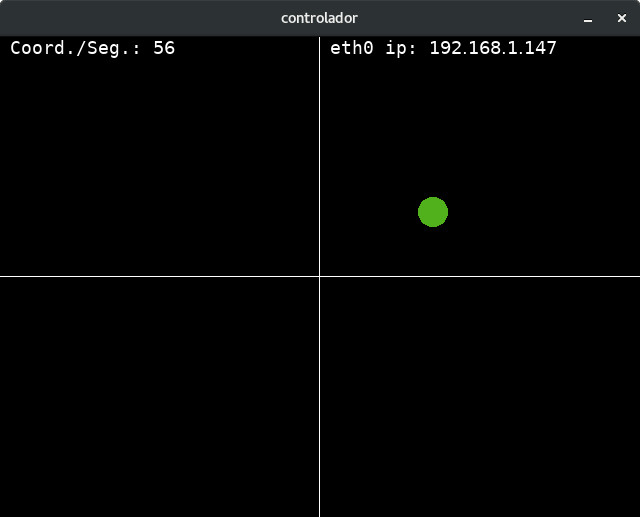
\includegraphics[width=0.95\textwidth]{figuras/controlador2.jpg}
		\caption{gerando posição com o click do mouse.}
		\label{fig:controlador_teste_coordenada}
	\end{subfigure}
	\caption{Captura de tela de depuração e teste dos motores do software de controle.}
\end{figure}

No modo de depuração, é mostrada uma tela com um painel negro e quatro quadrantes indicando a posição da câmera, através de um ponto branco (localizado no centro dos quadrantes, quando o programa inicia); um indicador, contendo a contagem de coordenadas recebidas por segundo (no canto superior esquerdo) e o endereço IP que está associado a interface de rede do \textit{Raspberry Pi} (no canto superior direito), ilustrado na \autoref{fig:controlador_teste} e na \autoref{fig:controlador_teste_coordenada}. \par

Através dessa interface é possível simular posições da câmera usando o mouse. Para isso, o circulo branco deve ser clicado e arrastado para uma posição qualquer dos quadrantes. Ao arrastar e soltar o ponto branco, uma coordenada relativa a posição do ponto na tela é calculada e enviada para os motores, ilustrado na \autoref{fig:controlador_teste_coordenada}.\par

Quando o ponto é movido no sentido horizontal, o motor horizontal é acionado, e de forma semelhante, quando o ponto se move na direção do eixo vertical, o motor vertical é acionado.\par

As coordenadas do ponto branco são capturadas em relação a sua posição, em \textit{pixels} horizontais e verticais, dentro do painel negro, sendo a coordenada (0;0) a menor possível, localizada no canto superior esquerdo, ilustrado na \autoref{fig:sistcoord0x0}, e a coordenada (640, 480) a maior possível, localizada no canto inferior direito do painel negro, ilustrada na \autoref{fig:sistcoord100x100}.\par

O programa de teste também possui uma função de demonstração, que gera coordenadas de forma automática para os motores servo. A câmera segue o padrão de movimento definido por uma função seno, que varre os limites verticais e horizontais da interface, isto é, o padrão de movimento começa na coordenada (0;50) e oscila como uma senoide até a coordenada (100;50). Quando o movimento chega ao limite horizontal, a função é invertida e a câmera volta ao ponto de origem, conforme ilustrado na \autoref{fig:camdemo}. O modo de demonstração pode ser ativado através da diretiva \textit{\textbf{\#define CAMDEMO}} ou diretamente pelo \textit{script} \textit{Makefile} passando o parâmetro \textbf{\textit{CFLAGS=-CAMDEMO}}.

Conforme explicado na \autoref{sec:pwm}, os motores servos deslocam seu eixo de acordo com a largura do pulso, enviado para seu controlador interno. Entretanto, as coordenadas simuladas pela interface de depuração e as que são recebidas do modulo \textit{Android}, não possuem a informação de largura de pulso ou quantidade de ângulos que determinado motor deve ser movimentado. Para resolver esse problema, foi proposto um sistema de posição independente da quantidade de \textit{pixels}, largura de pulso ou ângulos.\par

\begin{figure}[H]
	\centering
	\begin{subfigure}{.5\textwidth}
		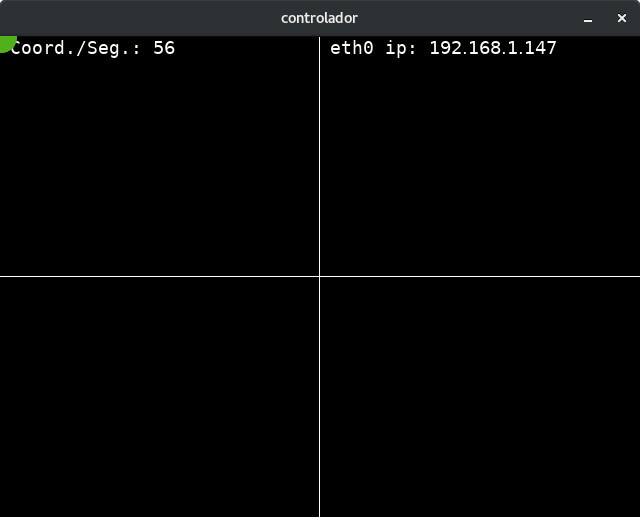
\includegraphics[width=0.95\textwidth]{figuras/controlador0x0.jpg}
		\caption{coordenada mínima}
		\label{fig:sistcoord0x0}
	\end{subfigure}%
	\begin{subfigure}{.5\textwidth}
		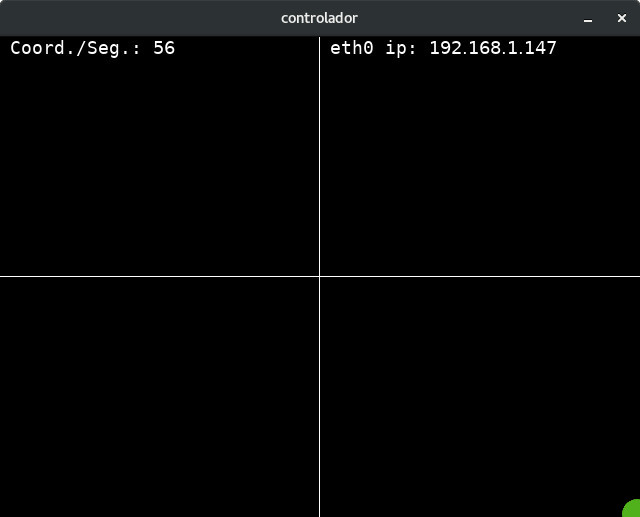
\includegraphics[width=0.95\textwidth]{figuras/controlador100x100.jpg}
		\caption{coordenada máxima}
		\label{fig:sistcoord100x100}
	\end{subfigure}

	\begin{subfigure}{.5\textwidth}
	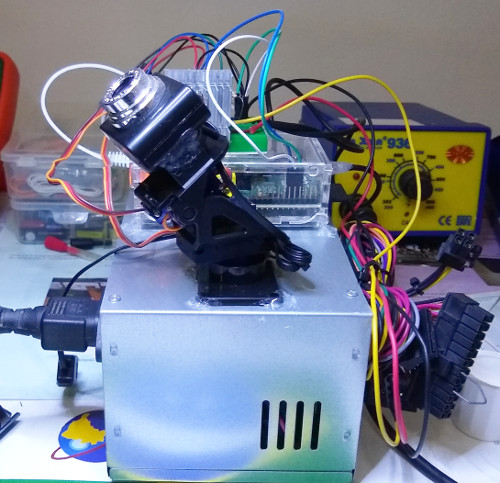
\includegraphics[width=0.95\textwidth]{figuras/camera0x0.jpg}
	\caption{reflexo da coordenada mínima na câmera}
	\label{fig:camera0x0}
	\end{subfigure}%
	\begin{subfigure}{.5\textwidth}
		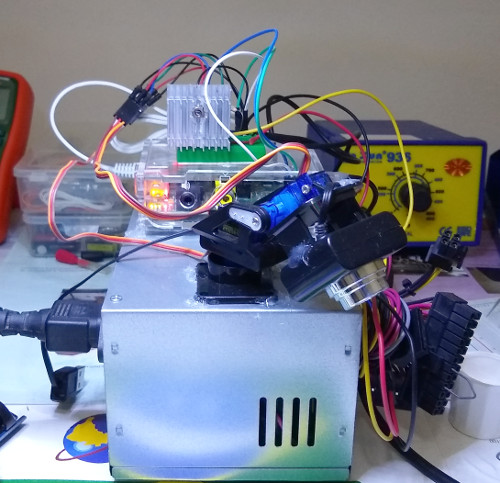
\includegraphics[width=0.95\textwidth]{figuras/camera100x100.jpg}
		\caption{reflexo da coordenada máxima na câmera}
		\label{fig:camera100x100}
	\end{subfigure}


	\begin{subfigure}{.5\textwidth}
		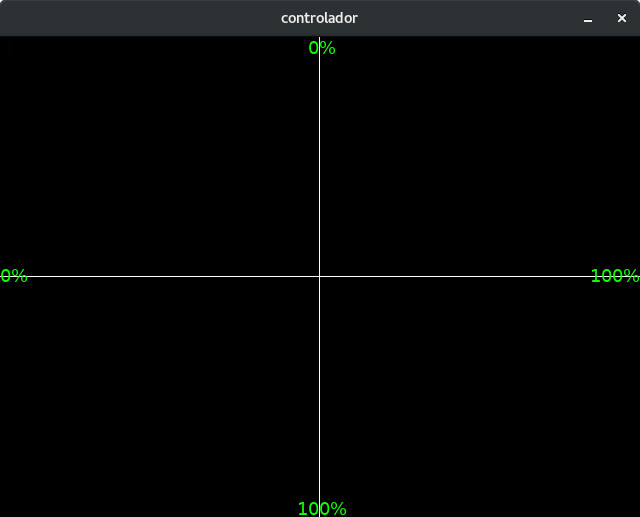
\includegraphics[width=0.95\textwidth]{figuras/controlador-values.jpg}
		\caption{orientação dos eixos.}
		\label{fig:sistcoord}
	\end{subfigure}
	\caption{Sistema de coordenadas proporcional.}
\end{figure}

O sistema de posição proposto é baseado na proporção, ou porcentagem, máxima do movimento possível (do motor, da cabeça do operador e do mouse no painel do programa de teste). Desse modo, o ângulo máximo que o motor horizontal, e a cabeça do operador, podem deslocar é $180\degree$, sendo $90\degree$ para a esquerda e $90\degree$ para a direita (partindo-se do ângulo $90\degree$, local de descanso do motor e centro de visão do operador), e está relacionado diretamente ao valor máximo de \textit{pixels} que a componente $x$ da coordenada de posição pode assumir, 640 \textit{pixels}, sendo 320 para a esquerda e 320 para a direita (partindo-se do centro da interface). De forma semelhante, movem-se no eixo vertical, o motor e a cabeça do operador com angulo máximo de $180\degree$, mudando apenas a quantidade máxima de \textit{pixels} na interface de teste, que nesse caso é 480, sendo 240 para cima e 240 para baixo.\par
A relação entre a largura de pulso enviada para os motores horizontal e vertical, em porcento, é dada respectivamente por:
\begin{equation}
	PWM_H = \frac{TARGET_X \times 100}{WIDTH}
	\label{eq:pwm_screen_h}
\end{equation}

\begin{equation}
	PWM_V = \frac{TARGET_Y \times 100}{HEIGHT}
	\label{eq:pwm_screen_v}
\end{equation}

Sendo $WIDTH = 640$ e $HEIGHT = 480$, a largura e altura do painel de teste; $TARGET_X$ e $TARGET_Y$ a localização real em \textit{pixels} horizontais de verticais do circulo indicador.

A \autoref{fig:sistcoord} mostra que o valor dos componentes das coordenada crescem, no sentido esquerda-direita horizontalmente e cima-baixo verticalmente. Como o sistema está expresso em porcentagem, os valores das coordenadas são enviados diretamente para os motores, como será visto adiante, no final da \autoref{subsec:deiverpwm}.\par

Um ajuste foi feito nas coordenadas que são enviadas para o motor servo que movimenta a câmera horizontalmente. Devido a montagem do motor inverter a posição do seu eixo, as coordenadas enviadas pela interface de depuração e pelo MCM foram invertidas, sendo assim a \autoref{eq:pwm_screen_h} foi ajustada para:

\begin{equation}
	PWM_H = 100 - (\frac{TARGET_X \times 100}{WIDTH})
	\label{eq:pwm_screen_h_inverse}
\end{equation}

Na \autoref{fig:sistcoord0x0} é possível visualizar o marcador de posição em verde, na posição (0;0), selecionado manualmente com o mouse, e seu reflexo nos motores, mostrado na \autoref{fig:camera0x0}. O mesmo acontece com o ponto máximo, ilustrado na \autoref{fig:sistcoord100x100} e o reflexo da seleção nos motores, na \autoref{fig:camera100x100}.\par

\subsection{Driver PWM}
\label{subsec:deiverpwm}

A geração de PWM pode ser realizada através de software ou hardware, usando um dispositivo especializado, implementado dentro do processador.\par

Testes foram feitos no inicio do projeto na expectativa de gerar um sinal PWM adequado via software, usando a biblioteca \textbf{RPi.GPIO} escrita em \textit{pyton}, já que a ideia inicial era escrever todos os módulos, inclusive o programa de testes, em \textit{pyton}. Entretanto, os resultados não foram satisfatórios. Os pulsos PWM gerados pela biblioteca não mantinham a frequência e nem a largura do pulso, causando um movimento errático dos motores. A partir desse teste, optou-se por utilizar a linguagem de programação C, nas bibliotecas e ao escrever o código dos softwares utilizados no \textit{Raspberry Pi}.\par

Outros testes foram feitos com uma biblioteca chamada \textbf{WiringPi}, escrita usando a linguagem C. A biblioteca não oferecia um bom suporte para PWM, sendo mais utilizada para controle geral dos pinos de propósito geral do \textit{Raspberry Pi}, e portanto foi descartada.\par

A biblioteca \textbf{bcm2835} também foi testada. Observou-se que é uma biblioteca muito extensa e oferece suporte aos diversos dispositivos de hardware como SPI, I2C e PWM, disponíveis no \textit{Raspberry Pi}. Entretanto, por não possuir uma documentação intuitiva e devido a sua complexidade associada ao curto tempo para a conclusão do projeto, sua utilização também foi descartada.\par

Por fim, o método utilizado para gerar um PWM estável, de forma rápida e confiável foi através do utilitário \textbf{ServoBlaster}, um software que provê uma interface de controle do \textit{driver} PWM, via árvore de dispositivos do sistema operacional \textit{Linux}. Sendo assim, através de um dispositivo localizado em \textbf{/dev/servoblaster}, foi possível gerar sinais PWM estáveis, para múltiplos pinos do \textit{Raspberry Pi}.\par 

Para acionar o \textit{driver} PWM basta abrir o dispositivo \textbf{/dev/servoblaster}, como um arquivo, e escrever os comandos de acionamento dos motores.\par

O utilitário \textbf{ServoBlaster} é instalado como um serviço no sistema operacional e fica esperando comandos serem escritos no dispositivo \textbf{/dev/servoblaster}, criado durante a instalação. Os comandos de acionamento dos servos são intuitivos e não é necessário conhecimento aprofundado em servo motores ou na eletrônica por trás da geração de PWM. Como exemplo, para mover um motor servo qualquer, conectado a um pino $X$ do \textit{Raspberry Pi}, para a posição $90\degree$, seu centro ou ponto de descanso, basta usar um emulador de terminal, como o \textit{bash}, e digitar o comando \textbf{echo X=50\% > /dev/servoblaster}; para mover o mesmo motor para sua posição inicial, ou $0\degree$, basta digitar \textbf{echo X=0\% > /dev/servoblaster}, e assim sucessivamente para qualquer ângulo $\theta$, sendo $0 \le \theta \le 180$.\par

O MCC usa o utilitário \textit{servoblaster} conforme descrito anteriormente, porém acessando o dispositivo \textbf{/dev/servoblaster} diretamente, isto é, através das funções de manipulação de arquivo (\textit{open} e \textit{write}), fornecidas pela API C básica do \textit{Linux}, a \textit{stdlibc}.

\subsection{Servidor de Imagens}
\label{subsec:mediaserver}

O MCC também é responsável por enviar as imagens da câmera, em tempo real, para o MCM. Com esse objetivo, testes foram feitos com a \textit{GStreamer}, uma biblioteca bastante utilizada na criação e manipulação de som e video no ambiente \textit{Linux}. Contudo, devido a uma incompatibilidade do sistema operacional utilizado no \textit{Raspberry Pi} e a biblioteca, a \textit{GStreamer} não foi adotada.\par

O VLC (\textit{VideoLAN Client}), um \textit{player} bastante difundido e multi-plataforma, com suporte a vários formatos de som e imagem, capaz de realizar \textit{stream}, usando protocolos de tempo real, em modo \textit{headless} (sem carregar uma interface gráfica, via linha de comando) foi testado também. Entretanto, seu uso foi descartado por utilizar demasiadamente o processador (por volta dos 97\% de CPU e 71MB da memória RAM), possivelmente causando comportamentos indesejados no controle dos motores.\par

Testes foram realizados também com o \textit{FFmpeg}, um utilitário multi-plataforma usado em manipulações de som e imagem, bastante versátil, com suporte a um grande número de \textit{codecs} e capacidade para realizar \textit{stream} de áudio e vídeo. O software foi recompilado para o \textit{Rasspberry Pi} com o objetivo de ativar seu suporte ao \textit{codec} de vídeo \textbf{h264\_omx}, implementado em hardware, no chip de silício que contem o processador e todos os periféricos do \textit{Raspberry Pi}, visando reduzir o uso do processador para tarefas de decodificação do vídeo. Por apresentar melhor desempenho (em média 70\% do uso do CPU e 46MB de memória RAM), esse utilitário foi usado para enviar o vídeo para o MCM.



\subsection{Construção do Módulo de Captura de Movimento - MCM}
\label{subsec:assemmodcapmov}

O MCM é responsável por obter, filtrar e enviar coordenadas, relativas a posição da cabeça do operador, para o MCM. É formado por um software, programado em Java e roda num smartfone \textit{Android}, que possui uma interface intuitiva de operação, ilustrado na \autoref{fig:moduloandroid}, e um conjunto de sensores embutidos no celular, que são capazes de fornecer dados relativos a orientação com uma boa acuracidade. \par

O programa de captura de coordenadas pode ser resumido basicamente em quatro partes principais: \textbf{coleta de dados} de posição da cabeça do operador; \textbf{envio de coordenadas}; \textbf{interação com o operador} (interface do usuário); e, \textbf{exibição do vídeo} capturado pela câmera. Que serão detalhadas adiante, iniciando-se pela  interface com o usuário.\par


\begin{figure}[H]
	\centering
	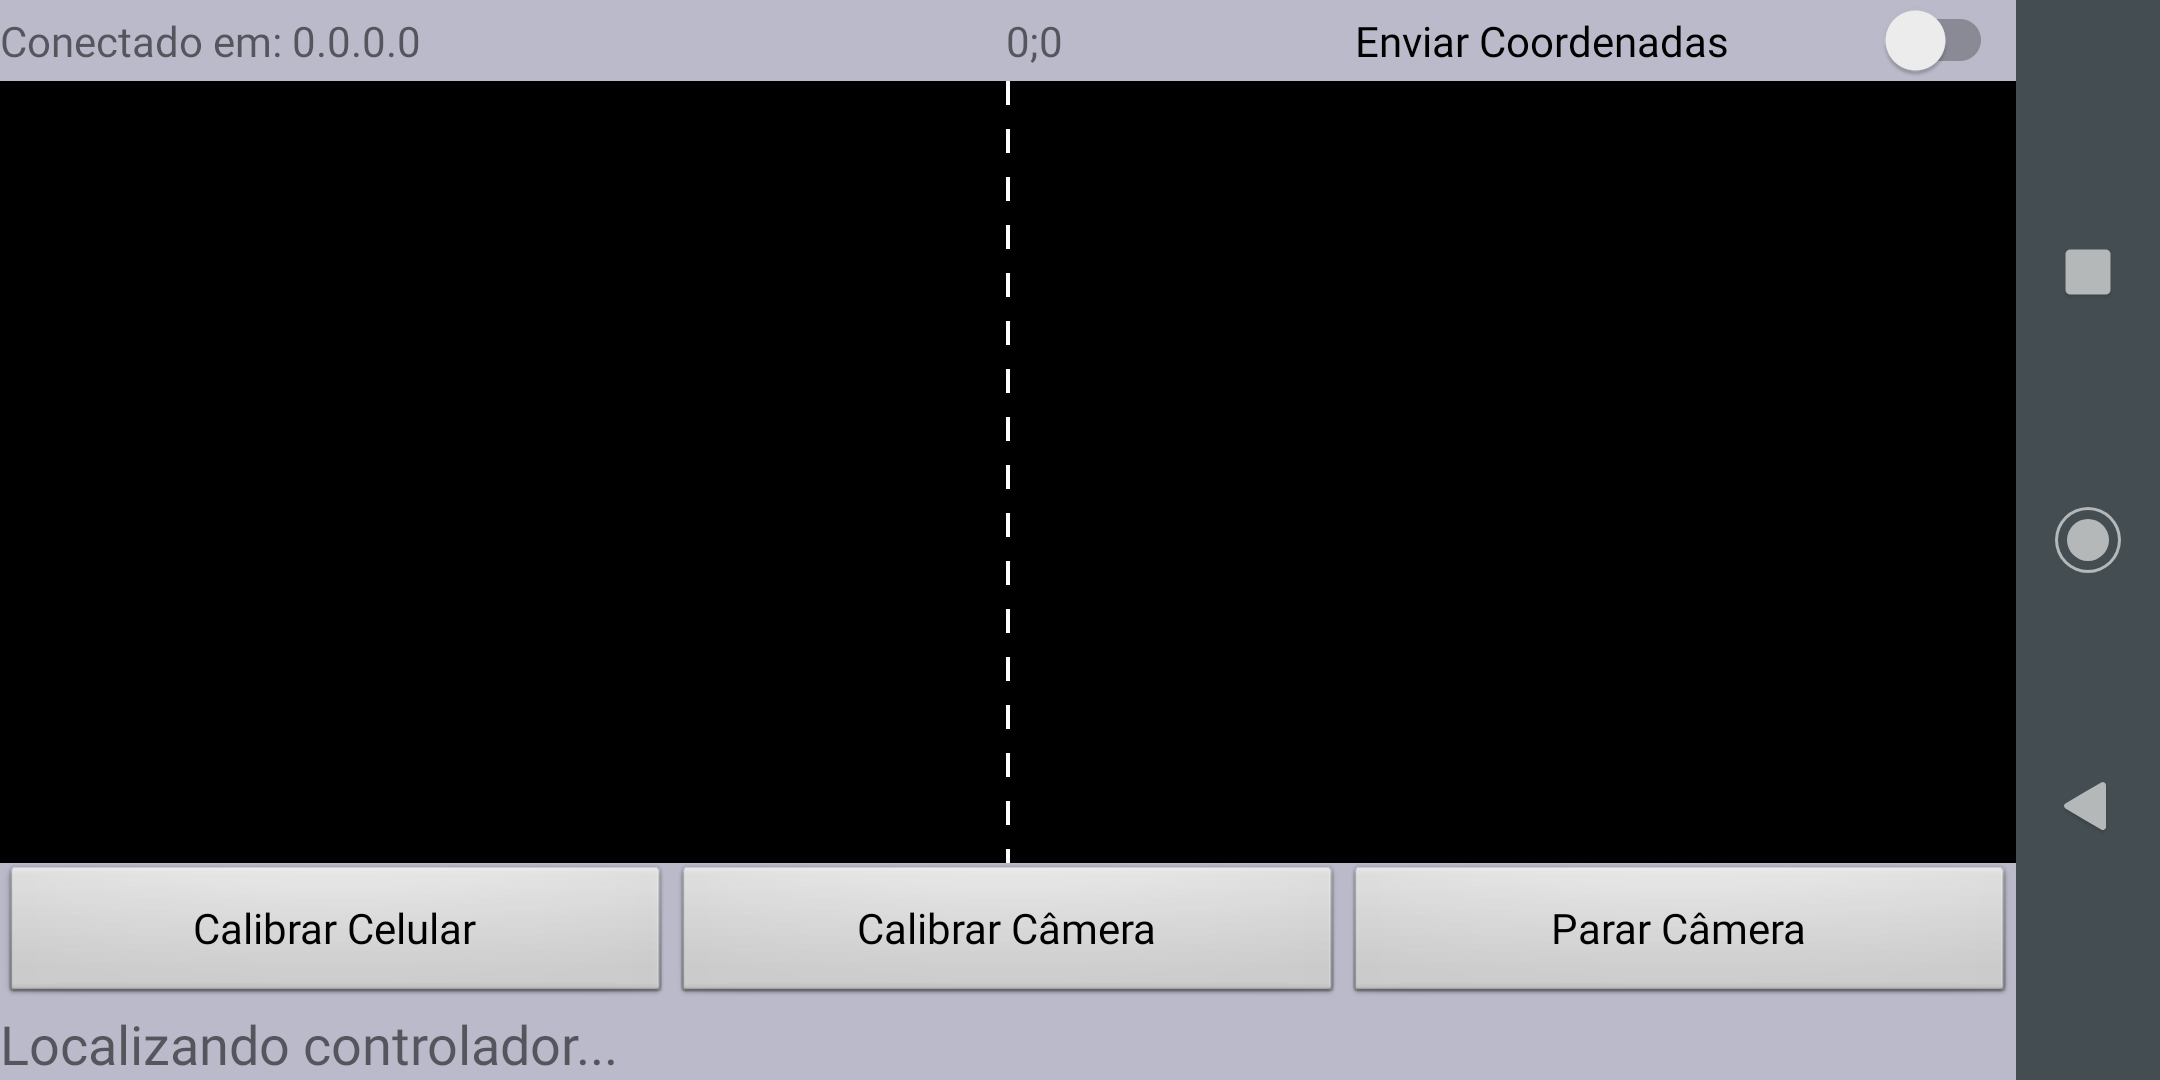
\includegraphics[width=1\textwidth]{figuras/modulo_android_1.png}
	\caption{Interface do Módulo de Captura de Movimento.}
	\label{fig:moduloandroid}
\end{figure}

A captura de tela da interface do MCM, ilustrada na \autoref{fig:moduloandroid}, mostra uma serie de componentes visuais, que trazem informações pertinentes ao funcionamento do sistema e permitem interagir remotamente com o MCC. \par

O \textbf{indicador de conexão}, localizado no canto superior esquerdo da interface, indica a qual endereço IP está associado ao servidor, responsável por controlar os motores que movimentam a câmera, e ao mesmo tempo disponibilizam as imagens capturadas. Quando o valor mostrado é \textbf{0.0.0.0}, significa que está desconectado de um servidor e não será possível enviar coordenadas ou receber imagens.\par

O \textbf{indicador de coordenadas}, localizado na parte central superior da interface, indica qual coordenada está sendo capturada, em tempo real, pelos sensores de movimento do celular. Seu formato é semelhante a uma coordenada cartesiana, isto é, a componente da $x$ seguindo da componente $y$ e separada por um "ponto e virgula". Esse indicador mostra pontos do sistema de coordenadas proposto na \autoref{subsec:assemmodconcam}, desse modo, a coordenada \textbf{50;50} é equivalente ao centro da interface de depuração.\par

No canto superior direito da interface, se encontra o \textbf{controle de envio de coordenada}, uma chave do tipo \textit{on-off} que somente é habilitada quando o Módulo de Captura de Movimento está conectado a um servidor de controle de câmera. Quando a chave está na posição \textit{on}, ou ativada, as coordenas são enviadas para o servidor de controle de câmera.\par

Ao centro da interface, numa área em cor preta, está localizado o \textbf{painel de imagens}. Este é o local onde as imagens da câmera são mostradas quando recebidas do módulo de controle de câmera. O painel de imagens é dividido, verticalmente ao centro em duas porções, indicado pela linha tracejada em cor branca.\par

A divisão é devida ao sistema de vídeo \textit{stereo} simulado, onde uma única imagem enviada pelo módulo de controle de câmera é duplicada e manipulada de forma a criar um efeito \textit{parallax}, isto é, criar a sensação de que existem duas fontes de vídeo (duas câmeras), capturando imagens de um mesmo objeto a partir de ângulos de visão distintos, trazendo a sensação 3D para o operador.\par

A interface possui uma \textbf{barra de \textit{status}}, localizada na parte inferior, que indica qual tarefa está sendo executada no momento. A barra de \textit{status} mostrada na \autoref{fig:moduloandroid} indica que quando a imagem foi capturada o Módulo de Captura de Movimento estava buscando o Módulo de Controle de Câmera.\par

O mecanismo de busca do Módulo de Controle de Câmera se dá através do disparo em \textit{broadcast} de pacotes do tipo \textit{User Datagram Protocol}, mais conhecido como pacotes UDP, com uma mensagem especifica, somente respondida pelo Módulo de Controle de Câmera com o seu endereço IP associado. Desse modo, o Módulo de Captura de Movimento configura o endereço IP respondido como um Módulo de Controle de Câmera válido e habilita o controle de envio de coordenadas.\par

Acima da barra de \textit{status} e abaixo do painel de imagens, está localizado o menu de botões, contendo as funções de \textbf{calibração do celular}, que consiste em salvar as coordenadas referentes a posição atual do celular, usadas posteriormente para calcular uma nova coordenada ajustada que será enviada para o Módulo de Controle de Câmera; a função de \textbf{calibração de câmera}, que envia uma mensagem de calibração para o Módulo de Controle de Câmera para salvar a coordenada referentes a atual da câmera, usada posteriormente como referencia para movimentar a câmera; e, por fim, a função \textbf{Parar/Enviar Câmera}, que controla o envio de imagens do Módulo de Controle de Câmera.\par

Devido a escassez de recursos de hardware no Raspberry Pi (processador e memória RAM) associados a qualidade inferior da câmera utilizada no protótipo, a imagem capturada e enviada para o \textit{smartphone} tem péssima resolução (320x240 \textit{pixels}). Quando escalonada para preencher a área disponível na interface do celular, resultou numa figura desforme que pouco representa o objeto filmado. Sendo assim, apenas uma imagem está sendo mostrada, em tamanho reduzido e fora de alinhamento com a interface, conforme ilustrado na \autoref{fig:moduloandroid_cam}. Também, devido aos mesmos problemas relacionados ao hardware e qualidade da câmera, existe um atraso de aproximadamente 4 segundos entre as imagens que são coletadas na câmera e as imagens que são exibidas no aplicativo do celular.

\begin{figure}[H]
	\centering
	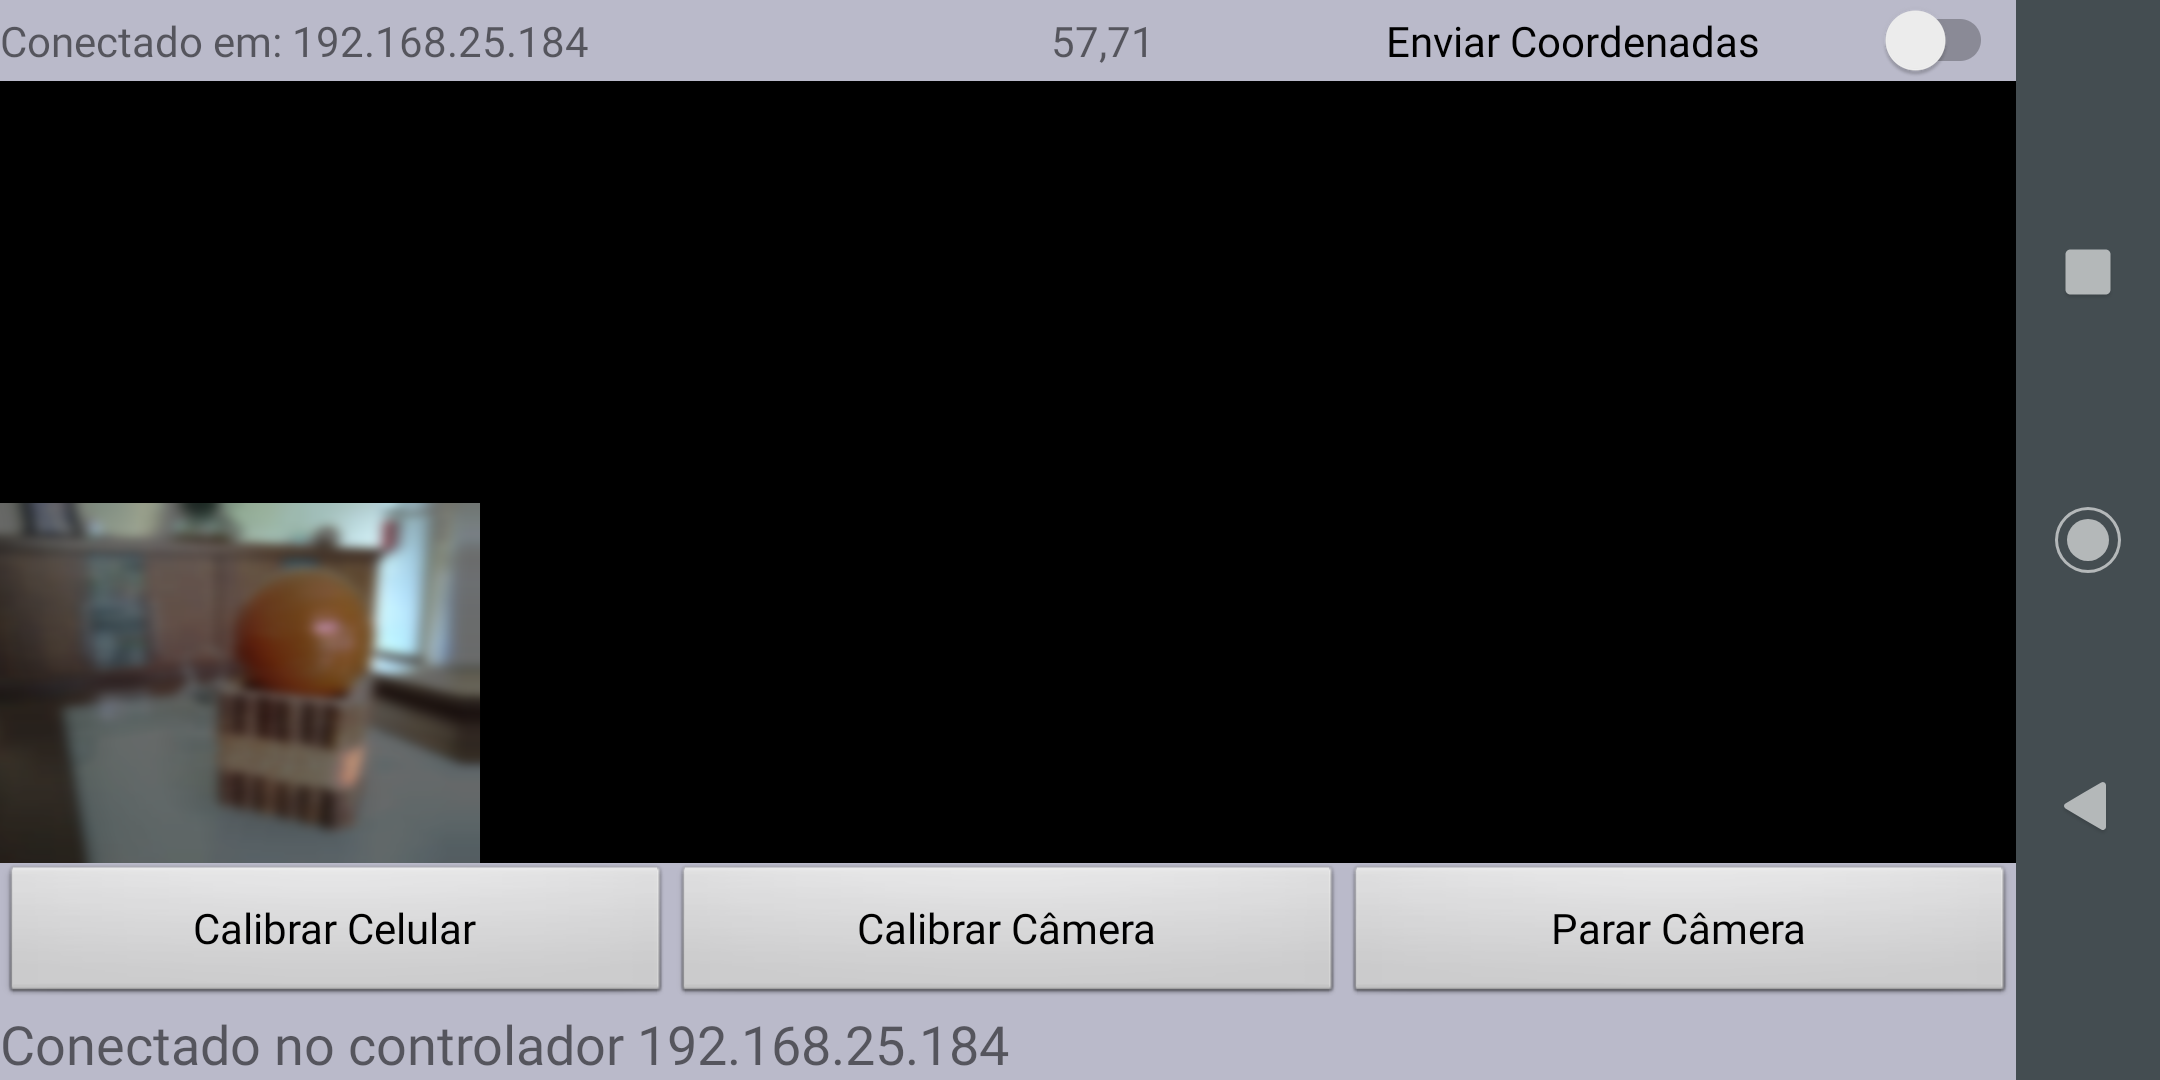
\includegraphics[width=1\textwidth]{figuras/modulo_android_2.png}
	\caption{Imagem da câmera em tamanho original.}
	\label{fig:moduloandroid_cam}
\end{figure}

Para mostrar as imagens capturadas pela câmera no celular e transmitida via RTP \textit{Real Time Protocol}, foi utilizado a biblioteca do \textit{VLC}, a mesma testada na \autoref{subsec:mediaserver}. Foi recompilada para o sistema operacional \textit{Android} e integrada ao programa de captura de movimento. Essa biblioteca foi selecionada para ser integrada por oferecer opções de compatibilidade com o sistema operacional \textit{Android}, ser compatível com diversos formatos de vídeo e ter suporte ao \textit{RTP}.\par

A coleta de dados de movimento, acontece a cada 30 milissegundos, através dos eventos de posição fornecidos pela API do sistema operacional \textit{Android}, que simplificam bastante o desenvolvimento de aplicações, abstraindo toda configuração do hardware dos sensores e a densa matemática, necessária para converter leitura de forças exercidas sobre o aparelho e interações dos vetores aceleração, em uma estrutura de dados que representa numericamente a posição espacial em que se encontra o celular. Contudo, é necessário identificar a orientação do aparelho, \autoref{fig:axisdevice}, em relação ao sistema de eixos do planeta, ilustrado na \autoref{fig:axisglobe} para que a coleta de dados funcione adequadamente.\par

O envio de coordenadas ocorre assim que um evento de posição é disparado. Ou seja, um novo envio de coordenada acontece a cada 30 milissegundos. Supondo que um par de coordenadas em média consuma 5 bytes (2 bytes para a coordenada $x$, 2 bytes para a coordenada $y$ e 1 byte para um caractere separador), seriam enviados 167 bytes por segundo, desconsiderando o \textit{overhead} do protocolo TCP (\textit{Transmission Control Protocol}), usado para esta finalidade. O consumo da banda de dados, gerado pela transmissão das coordenadas, pode ser considerado irrisório para um \textit{link} de 100Mbit/s, atualmente comum em redes do tipo \textit{Ethernet}. Entretanto, visando reduzir os recursos computacionais do celular, e consequentemente economizar bateria, um filtro verifica se houve mudança nas coordenadas antes de enviá-las, reduzindo o uso da banda de dados para aproximadamente 7 \textit{bytes} por segundo.\par

  